\chapter{Fusing Acoustic and Linguistic Information at Decision Level}
\chaptermark{Decision-level fusion}

This chapter evaluates the fusion of acoustic and linguistic information at the
decision level to improve speech emotion recognition (SER) performance. The
evaluated method consists of two stages. First, deep neural networks (DNNs)
process the unimodal training data from each modality to predict the output
(emotion degrees) of development/validation data. Second, the outputs of DNNs
from acoustic and linguistic networks are fed into SVM to obtain the final
prediction of emotion degrees. 

\section{Datasets partition}
Since this study also evaluates some conditions of the dataset (semi
lexical-controlled data, speaker dependent vs. speaker independent), the
datasets are split into four partitions or scenarios.  Two datasets were
used in this part of the study. The first is the IEMOCAP dataset, which was
used in the previous chapters. The dimensional labels are valence (V), arousal
(A), and dominance (D) in a 5-point integer scale.  However, it was found that
some labels have values lower than 1 (e.g., 0.5) and higher than 5 (e.g., 5.5).
These outliers were removed; the remaining data were converted from a
5-point scale to [-1, 1] scale.

In addition to IEMOCAP dataset, MSP-IMPROV dataset \cite{busso2016msp} was
used.  The MSP-IMPROV dataset was designed within a dialogue framework to
elicit target sentences with the same semantic content but was produced with
different emotional expressions. In one recording, the target sentences were
produced ad-lib; for another recording, the target sentences were read.  These
two recordings are referred to as ``Target-improvised" and ``Target-read",
respectively. Since the goal is to examine the effect of both linguistic and
acoustic information on emotional ratings at the late-fusion stage, these
recordings were not appropriate for this study. However, two sets of
recordings, which did not have the same semantic content, were used, called
``Other-improvised" and ``Natural-interaction." The former included
conversations of the actors during improvisation sessions; the latter included
the exchanges during the breaks. This natural-interaction is recorded while the
actors were not acting. Zhang et al. \cite{ Zhang2019} used a similar protocol,
and this study followed their lead in referring to this subset of the
MSP-IMPROV dataset as MSP-I+N (MSP improvised and natural interaction) or
MSPIN. In this work, the same text transcriptions used by Zhang et al. was used
(the authors of the dataset provide transcriptions); for the additional
utterances not included in the Zhang study, transcriptions were obtained using
Mozilla's DeepSpeech \cite{DeepSpeech2019}.  This study thus uses 7166
utterances from a total of 8438. The speech data in the dataset was sampled in
mono at 44.1 kHz, with one file per utterance/sentence.

This study split each dataset into two partitions to observe any differences
between a speaker-dependent (SD) partition and a speaker-independent partition
made by leaving one session out (LOSO) for each dataset. For example, for the
IEMOCAP dataset, the last session (i.e., session 5), recorded from two
different actors (out of 10), is only used for testing. Similarly, all
utterances from session 6 (two speakers out of 12) are used for the MSP-I+N
test set.  The rule for data splitting is to divide between the training +
development and test sets in a ratio close to 80:20. This rule applies to both
the SD and LOSO partitions. Then, of the training + development data, 80\% is
used for training, and the remaining 20\% is used for development, as shown in
Figure \ref{fig:data_partition}. Both methods are evaluated with the same
unseen test sets to compare the performance and measure the improvement. Note
that the dataset was not validated using a cross-validation technique (but
instead divided into training and test data) for evaluation since the number of
samples for both datasets is adequate (10039 and 7166 samples). This strategy
is also utilized to keep the same test set for LSTM (one-stage processing) and
SVM (two-stage processing) which is difficult if the samples are
shuffled/cross-validated.

\begin{figure}
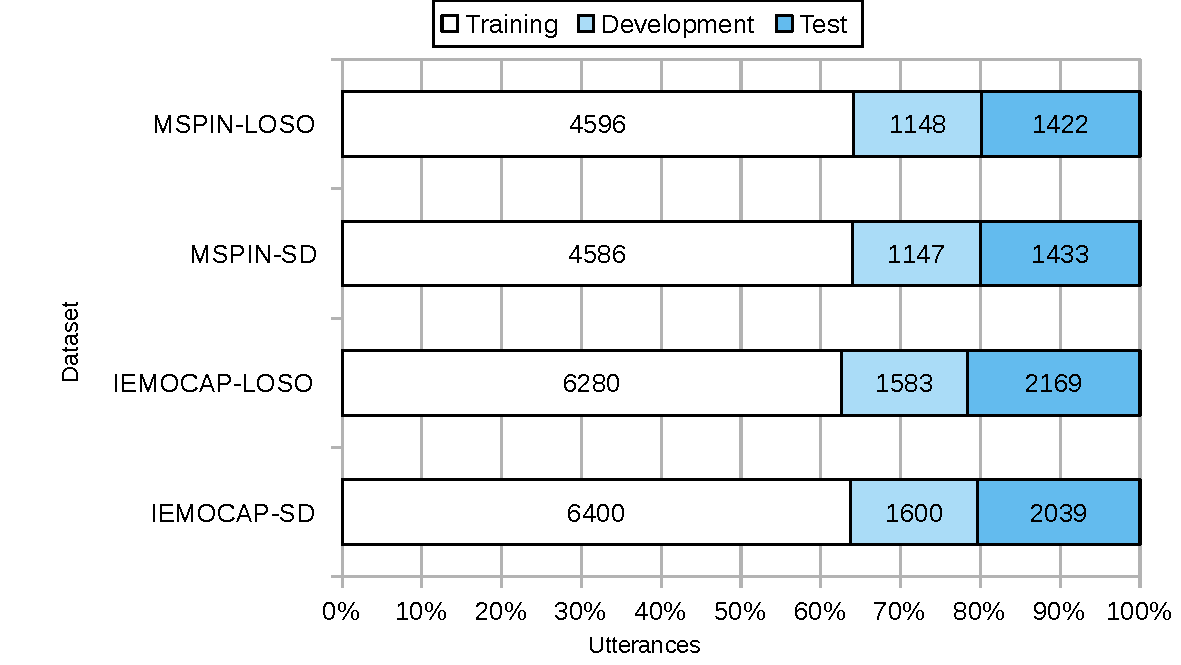
\includegraphics[width=6in]{../fig/csl_partition.pdf}
\caption{Proportion of data splitting for each partition of each dataset. In
one-stage LSTM processing, the outputs of the model are both development and
test data. In the second stage, i.e., the SVM processing, the input data is the
prediction from the development set of the previous stage, and the output is
the prediction of test data.}
\label{fig:data_partition}
\end{figure}

% \section{Introduction}
\section{Two-stage dimensional SER}
% Give a reason on why only choosing WE, word2vec, and GloVe The reason is
% Table 5.2, WE,word2vec, and GloVE achiece 1-3 best.

\subsection{LSTM network for unimodal prediction}
\subsubsection{Acoustic emotion recognition}

Based on the results on the previous early fusion method, it was found that
LSTM is more beneficial than CNN to model both acoustic- and
linguistic-based emotion recognition. The DNN at the first stage of the late
fusion approach adopts this LSTM network. The acoustic network receives input
in different acoustic features for evaluation. Not only differs in feature
sets, this evaluation continues the previous work \cite{Atmaja2020f} in the use
of different datasets.  Apart from the acoustic features used in the previous
chapter, this study evaluates three acoustic different feature sets: LLDs of
GeMAPS, Mean+Std features at the utterance level from these LLDs (HSF1), and an
additional silence feature with these statistical functions (HSF2).

The LLD features are the 23 acoustic features listed in Table
\ref{tab:aco_feature}. For each frame (25 ms), these 23 acoustic features are
extracted. With a hop size of 10 ms, the maximum number of sequences is 3409
for the IEMOCAP dataset and 3812 for the MSP-I+N dataset. Hence, the input size
is 3409 $\times$ 23 for IEMOCAP and 3812 $\times$ 23 for MSP-I+N. The
extraction process uses the openSMILE toolkit \cite{Eyben2016open}.

\begin{table}
\caption{Acoustic feature sets derived from the GeMAPS features by \cite{Eyben}
and the statistical functions used for dimensional SER in this research}
    \begin{center}
\begin{tabular}{p{6cm} p{4cm} p{4cm}}
    \hline
LLDs & HSF1 & HSF2 \\
\hline \hline
intensity, alpha ratio, Hammarberg index, spectral slope 0-500 Hz, spectral
slope 500-1500 Hz, spectral flux, 4 MFCCs, F0, jitter, shimmer,
harmonics-to-noise ratio (HNR), harmonic difference H1-H2, harmonic difference
H1-A3, F1, F1 bandwidth, F1 amplitude, F2, F2 amplitude, F3, and F3 amplitude.
& mean (of LLDs), standard deviation (of LLDs) & mean (of LLDs), standard
deviation (of LLDs), silence \\
    \hline
    \end{tabular}
    \end{center}
    \label{tab:aco_feature}
   \end{table}

Figure \ref{fig:acoustic_model} shows an overview of the acoustic network. DNN
with LSTM architecture is chosen because the number of training samples is
adequate ($> 5000$ samples). Furthermore, it shows promising results in the
previous research \cite{Schmitt2018}.  Before entering the LSTM layers, the LLD
features at the input layer are fed into a batch normalization layer to speed
up the computation process. The three subsequent LSTM layers are stacked with
256 nodes in each layer, following one of the configurations in
\cite{Abdelwahab2018}. Instead of returning the last LSTM layer's final output,
the networks were designed to return the full sequence and flatten it before
inputting it to three dense layers representing valence, arousal, and
dominance. The outputs of these last dense layers are then the predictions for
those emotional attributes, i.e., the degrees of valence, arousal, and
dominance in the range [-1, 1]. 

\begin{figure}[htpb]
    \centering
    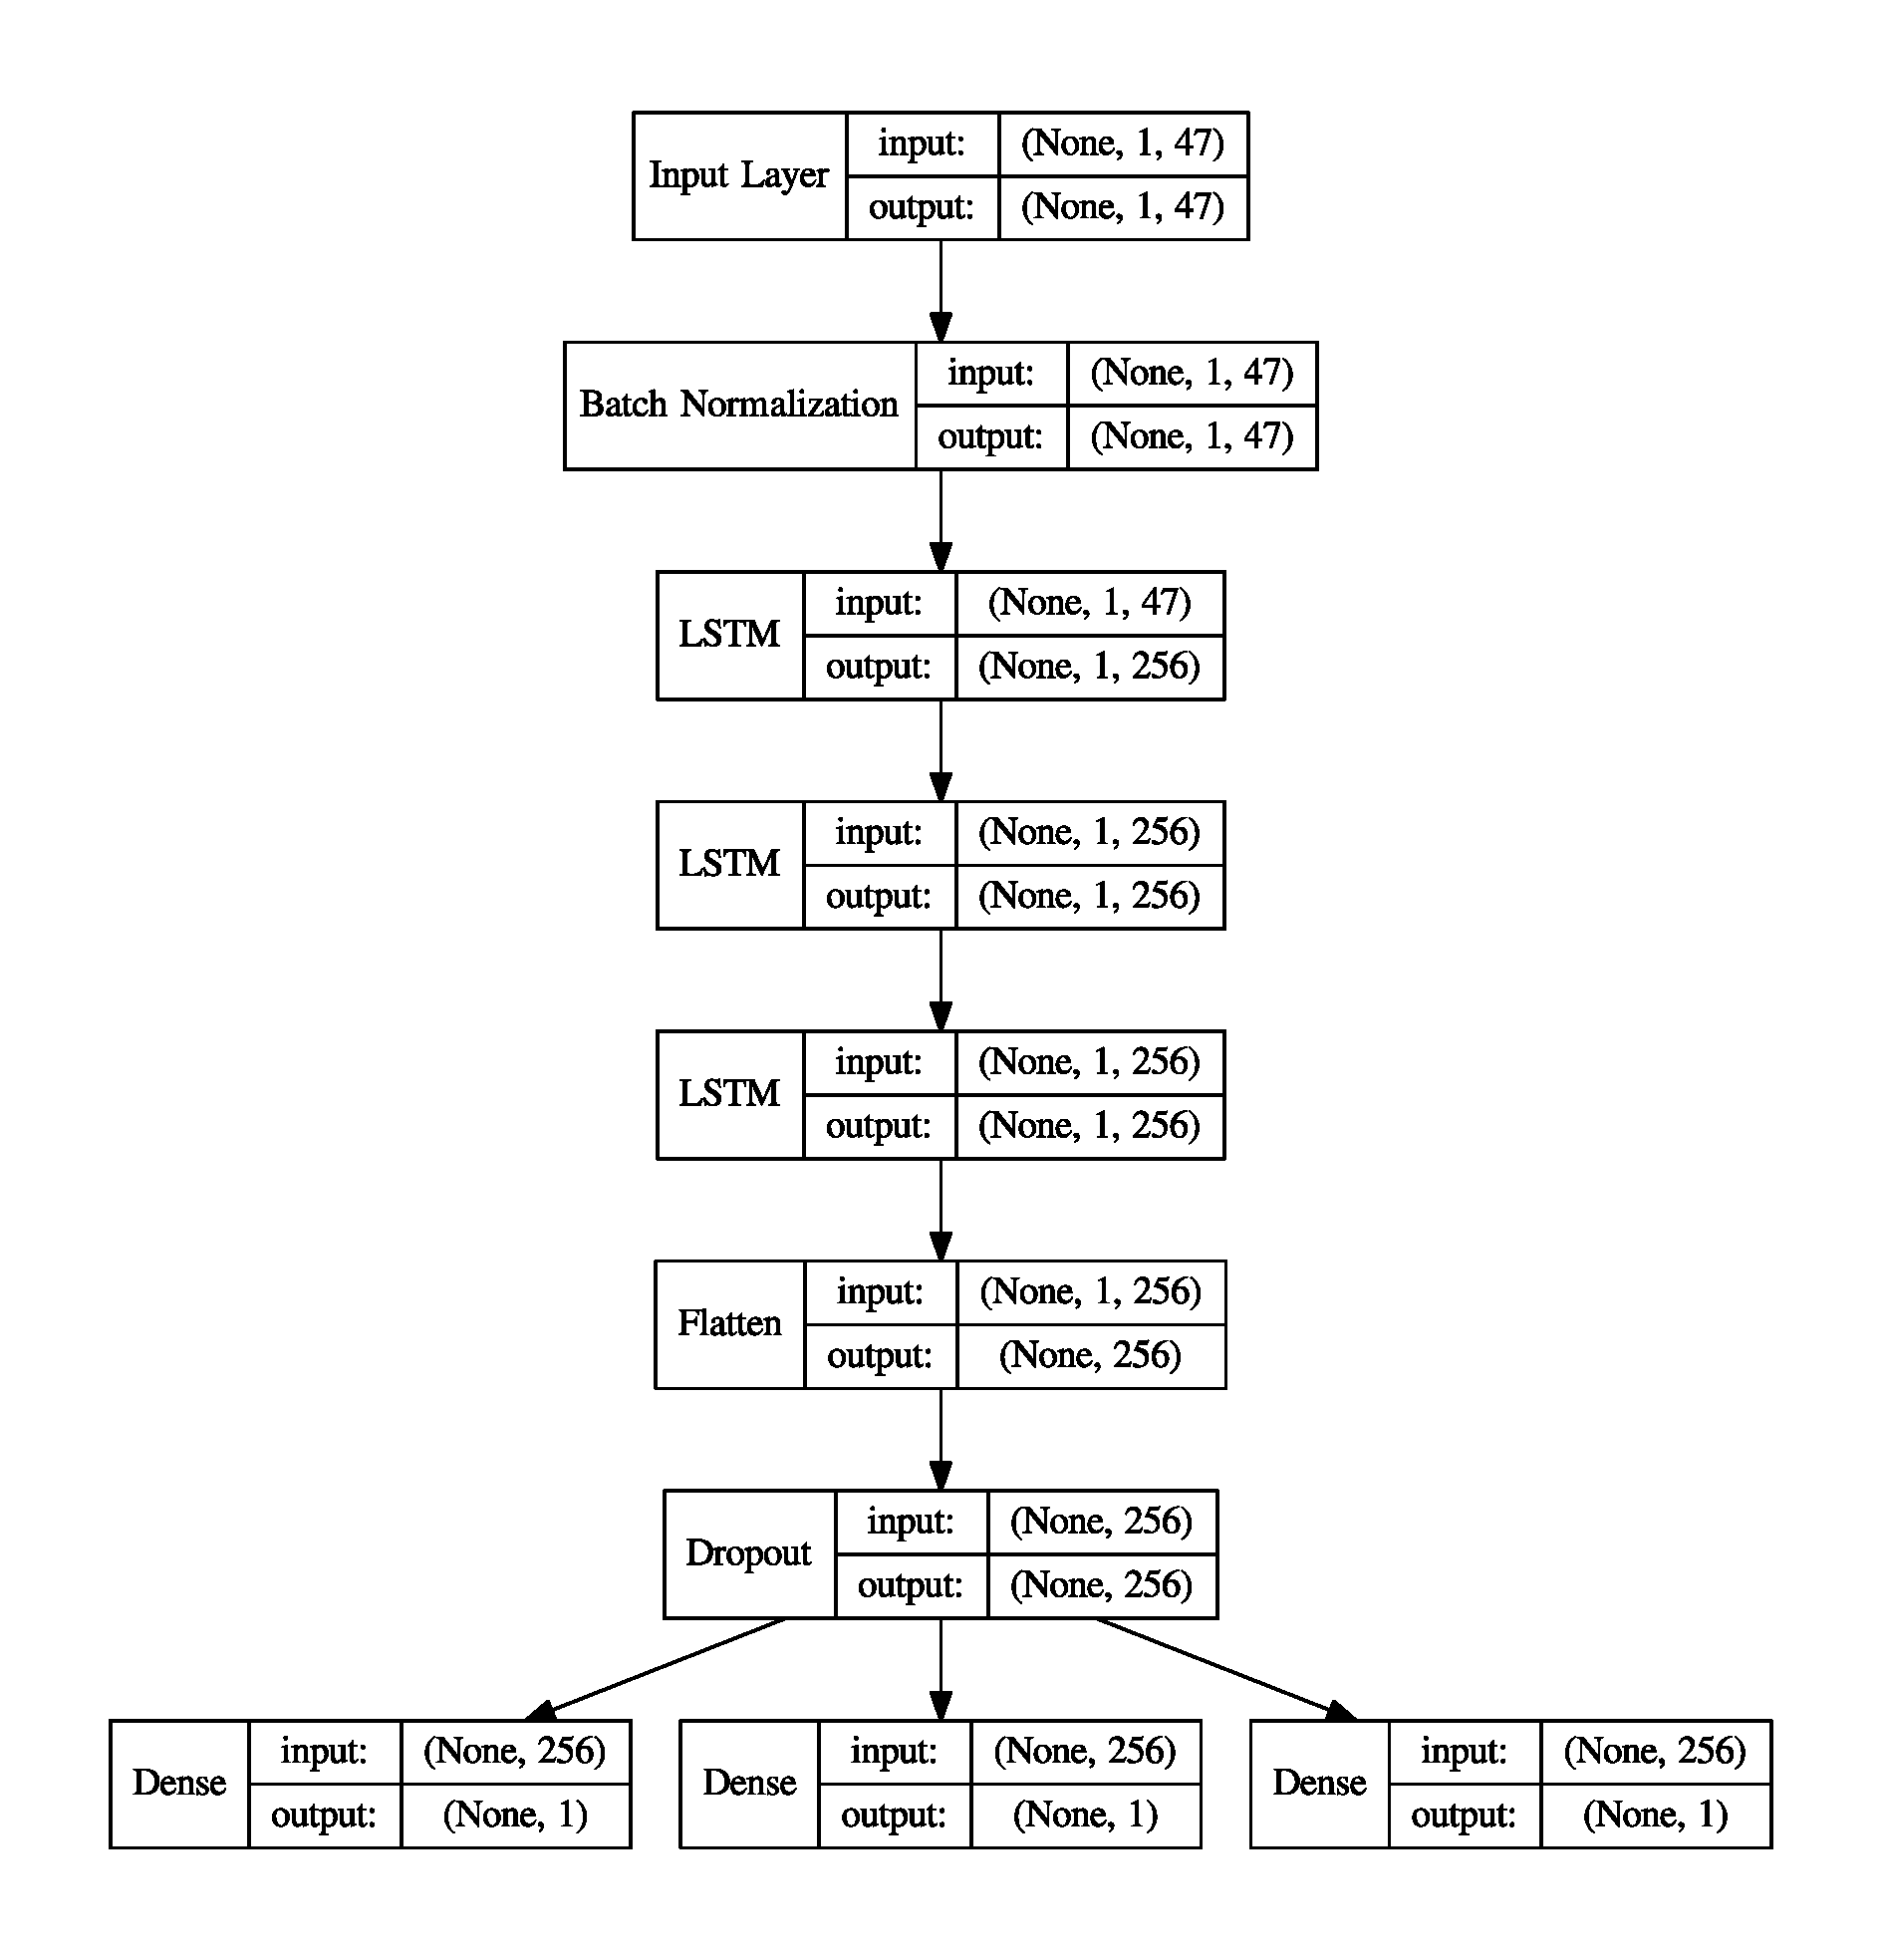
\includegraphics[width=0.8\textwidth]{../fig/model_acoustic.pdf}
    \caption{Structure of acoustic network to process acoustic features}
    \label{fig:acoustic_model}
    \end{figure}

The tuning of hyper-parameters follows the previous research
\cite{Atmaja2019b,Atmaja2020d}. A batch size of 8 was used with a maximum of 50
epochs. An early stop criterion with ten patiences would stop the training
process if no improvement was made in 10 epochs (before the maximum epoch) and
used the last highest-score model to predict the development data. An RMSprop
optimizer was used with its default learning rate, i.e., $0.001$. Table
\ref{tab:dnn_params} shows the setups on acoustic and linguistic networks. These
setups were obtained based on experiments with regard to the size of networks.
For instance, the smaller acoustic networks with HSF features employed $\tanh$
output activation function did not use the dropout rate while the larger
acoustic (with LLD) and linguistic networks employed linear activation
function and dropout rate.

\begin{table}
    \caption{The hyper-parameter used in experiments}
    \begin{center}
        \begin{tabular}{l| c c}
            \hline
Hyper-parameter  &  Acoustic network    & Linguistic network \\
\hline \hline
network type        &   LSTM            &   LSTM \\
number of layers    &   3               &   3 \\
number of units     &   256             &   256 \\
fourth layer        &   Flatten         &   Dense \\
hidden activation   &   linear          &   linear \\
output activation   & linear (LLD) / tanh (HSF)   &   linear \\
dropout rate        & 0.3 (LLD) / 0 (HSF)&   0.3 \\
learning rate       &   0.001           &   0.001  \\
batch size          &   8               &   8  \\
maximum epochs      &   50              &   50 \\
optimizer           &   RMSprop         &   RMSprop \\
            \hline
        \end{tabular}
    \end{center}
    \label{tab:dnn_params}
\end{table}

For the HSF1 and HSF2 inputs on acoustic networks, the same setup applies.
These two feature sets are very small as compared to the LLDs: HSF1 has a size
of 1 $\times$ 46, while HSF2 has a size of 1 $\times$ 47. This big difference
in input size (1:1800) leads to faster computation on HSF1 and HSF2 than on the
LLDs. Note that, although Figure \ref{fig:acoustic_model} shows HSF2 as the
input feature, the same architecture also applies for the LLDs and HSF1.

The idea of using LSTM is to hold the last output in memory and use that output
as a successive step. For instance, LLD with ($3409, 23$) feature size will
process the first time step 1 to the last time step 3409. For HSF1 and HSF2,
which contains a single timestamp, the data is processed only once ([1, 46] and
[1, 47] for HSF1 and HSF2). Here, the only difference, from multiple time
steps, is that the network performs three passes (forget gate, input gate, and
output gate) instead of a single pass (see \cite{Eyben2010}). This information
will include all information from the networks' memory.


\subsubsection{Linguistic emotion recognition}
The linguistic network, shown in Figure \ref{fig:text_model} for the MSP-I+N
dataset, use the same input size for the three different linguistic features.
The WE, WE with pre-trained word2vec, and WE with pre-trained GloVe embedding
were used on the basis of the previous results with 300 dimensions for each
word. The longest sequence in the IEMOCAP dataset is 100 sequences (words),
while for MSP-I+N, the longest is 300 sequences. Hence, the input feature sizes
for the LSTM layers are 100 $\times$ 300 for IEMOCAP and 300 $\times$ 300 for
MSP-I+N with its corresponding number of samples. The same three LSTM layers
are stacked as in the acoustic network, but the last LSTM layer only returns
the last output. A dense layer with a size of 128 nodes is added after the
LSTM layers and before the last three dense layers. Between the dense layers is
a dropout layer with the same probability of 0.3 to avoid overfitting.

\begin{figure}[htpb]
\centering
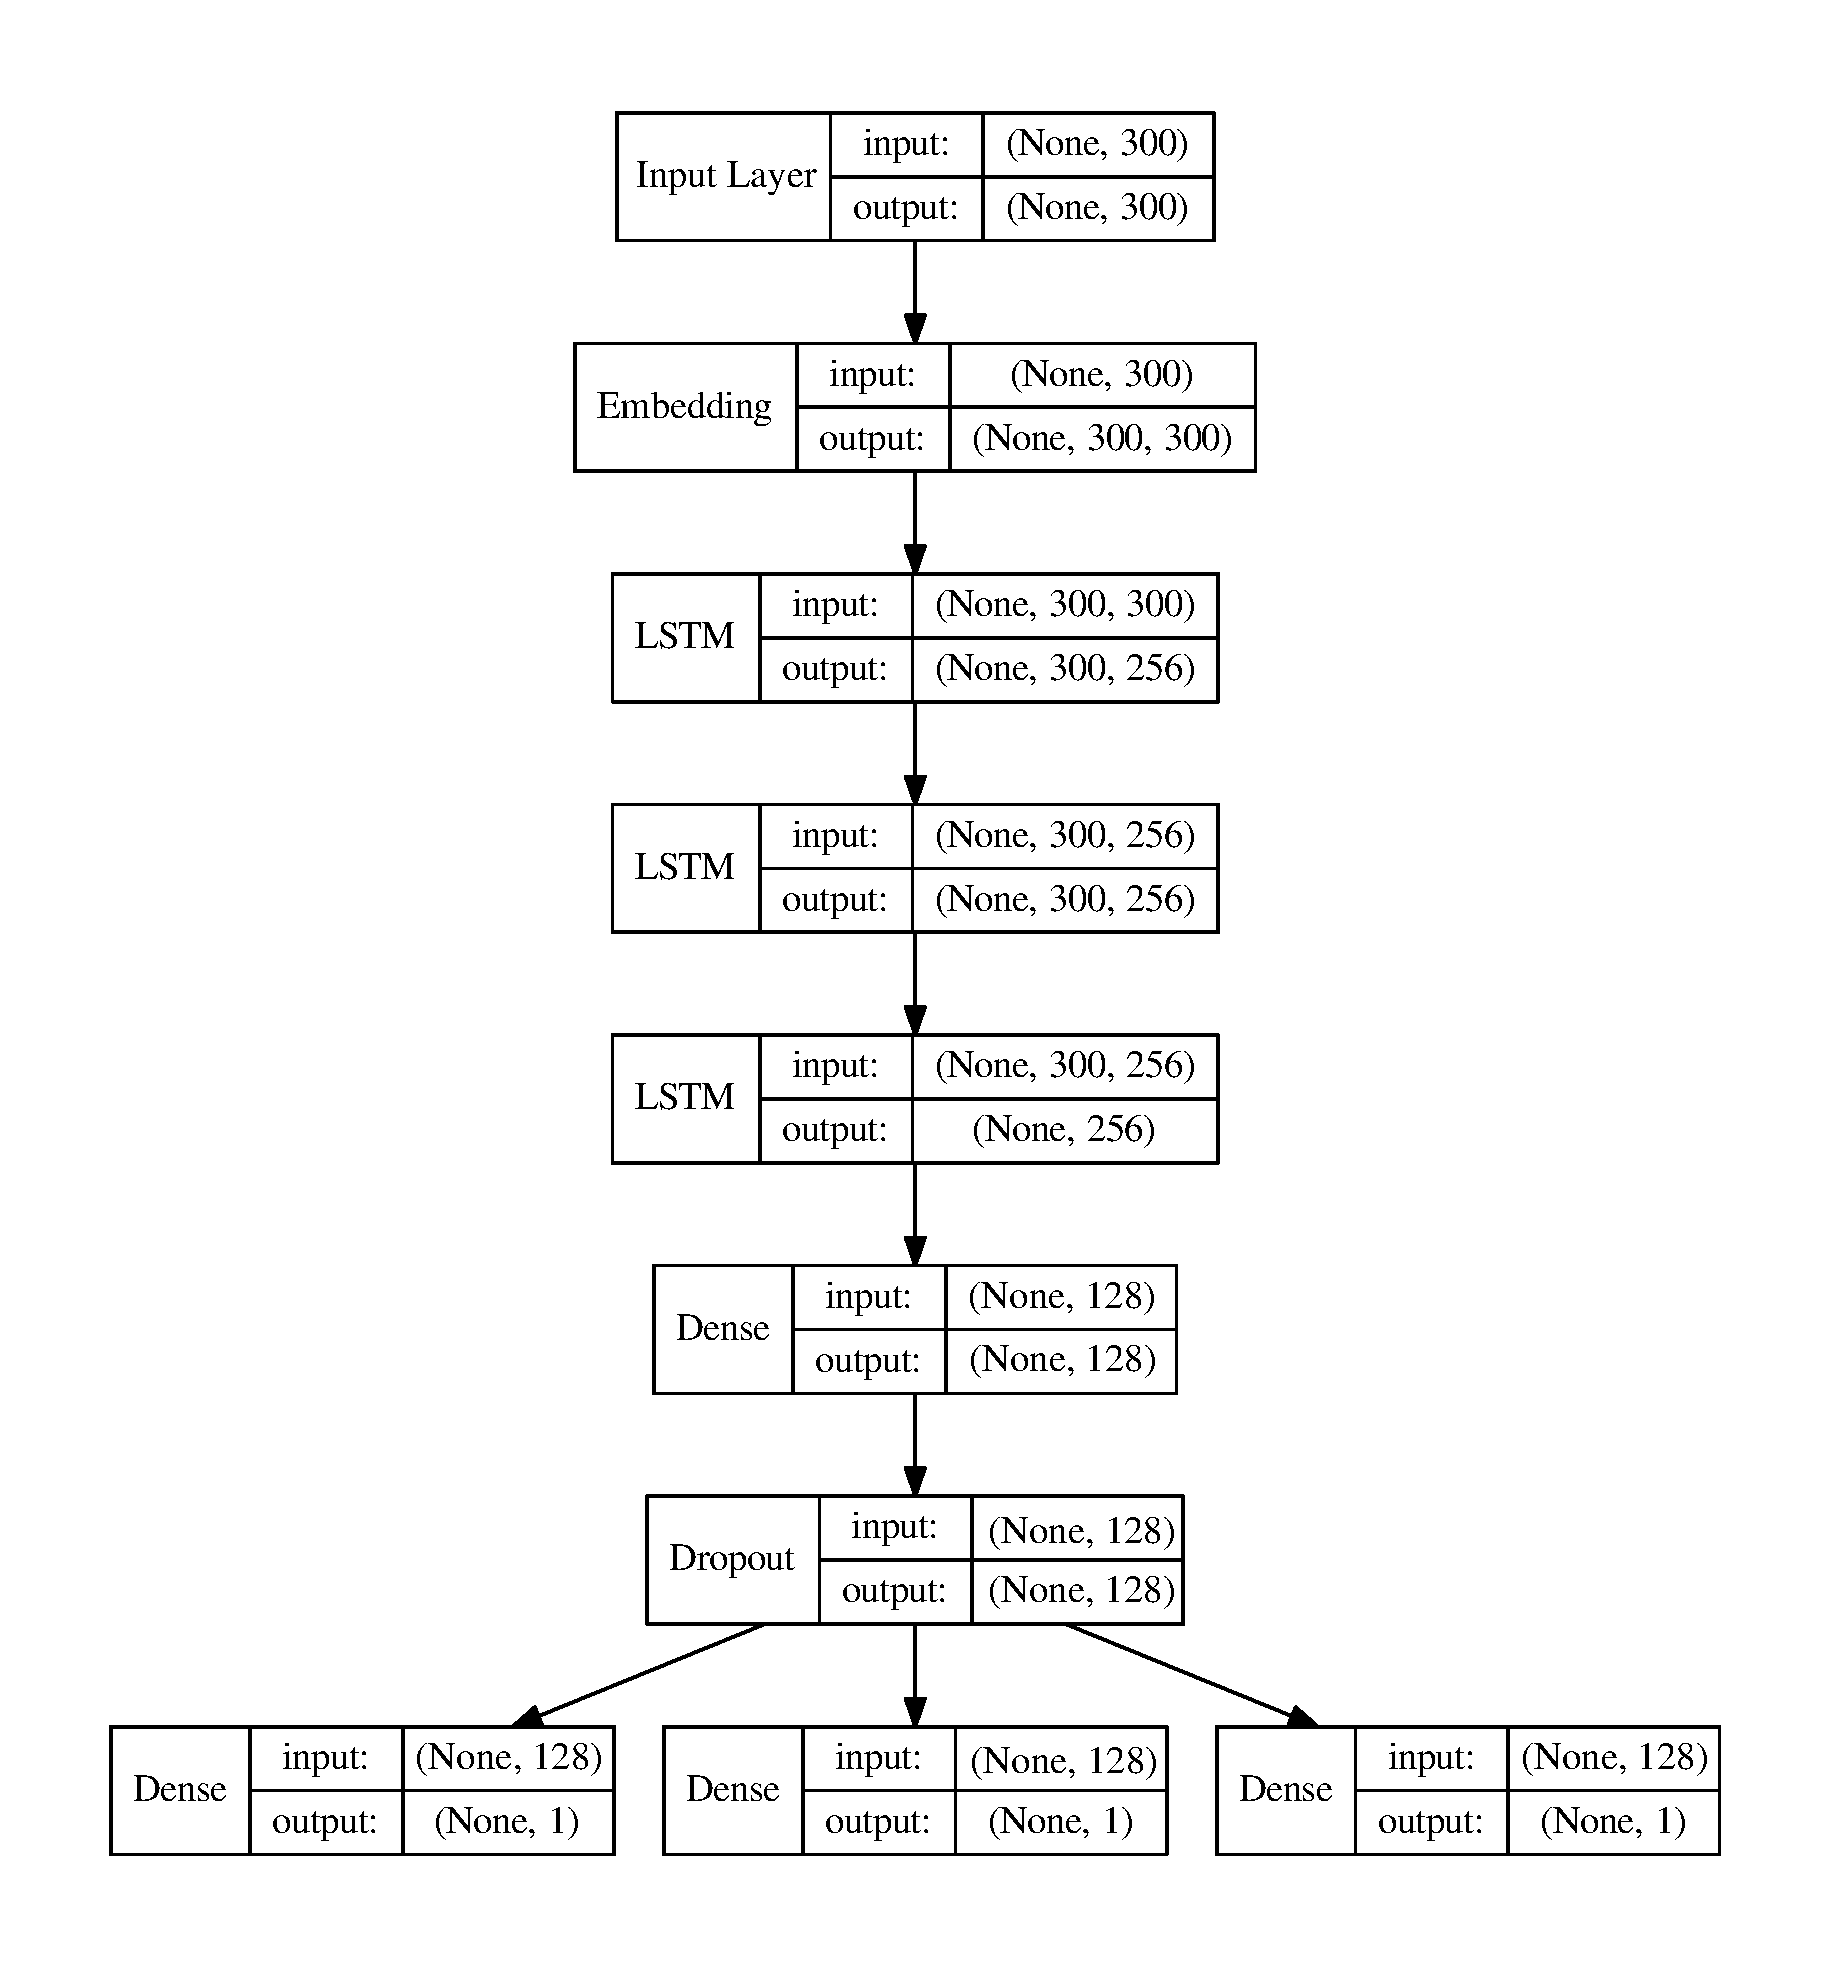
\includegraphics[width=0.8\textwidth]{../fig/model_text.pdf}
\caption{Structure of linguistic network to process word embeddings/vectors}
\label{fig:text_model}
\end{figure}

\subsection{SVM for results fusion}
The choice of an SVM (in this case, support vector regression, SVR) as the
final classifier to fuse the outputs of the acoustic and linguistic networks is
due to its effectiveness in handling smaller data (compared to a DNN) and its
computation speed. The data points produced by LSTM processing as the input of
SVM is small; i.e., 1600, 1538, 1147, and 1148 for IEMOCAP-SD, IEMOCAP-LOSO,
MSPIN-SD and MSPIN-LOS0, respectively. The SVM then applies regression analysis
to map them to the given labels. Figure \ref{fig:csl_system} shows the
architecture of this two-stage emotion recognition system using DNNs and an
SVM. Each prediction from the acoustic and linguistic networks is fed into the
SVM.  From two values (e.g., valence predictions from the acoustic and
linguistic networks), the SVM learns to generate a final predicted degree
(e.g., for valence). The concept of using the SVM as the final classifier is
summarized as Chapter 2.


\begin{figure}
\centering
 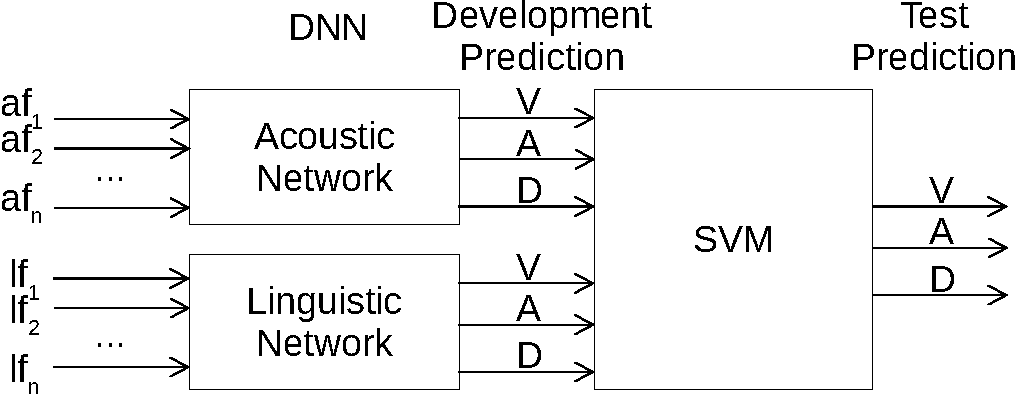
\includegraphics[width=0.9\textwidth]{../fig/csl_system-crop.pdf}
\caption{Proposed two-stage dimensional emotion recognition method using DNNs
and an SVM. The inputs are acoustic features (af) and linguistic features (lf);
the outputs are valence (V), arousal (A), and dominance (D).}
\label{fig:csl_system}
\end{figure}

\section{Results and discussion}
\subsection{Results from single modality}
Before presenting the bimodal feature-fusion results, it is important to show
the results of unimodal emotion recognition. The goals here are (1) to observe
the (relative) improvement of bimodal feature fusion over using a single
modality, and (2) to observe the effects of different features on different
emotion attributes.

Tables \ref{tab:ser-test} and \ref{tab:ter-test} summarize the single-modality
results of dimensional emotion recognition from the acoustic and linguistic
networks, respectively. In general, acoustic-based SER gave better results than
the text-based SER in terms of the average CCC score. For particular emotion
attributes, the linguistic network gave a higher CCC score for valence
prediction than those obtained by the acoustic network, except on the MSPIN
datasets. These results confirm the previous finding by \cite{Karadogan2012}
that valence is better estimated by semantic features, while acoustic features
better predict arousal. It is also found that acoustic features better
predicted the dominance dimension than linguistic features. This finding can be
inferred from both tables, in which the CCC scores for the dominance dimension
are frequently higher from the acoustic network than from the linguistic
networks.

The exception to a higher valence score on the MSPIN-SD dataset by the acoustic
networks can be seen as the effect of either the DNN architecture or the
dataset's characteristics. In \cite{chen2017multimodal}, the obtained score was
higher for valence than for arousal or liking (the third dimension, instead of
dominance) with their strategy on acoustic features. In contrast,
\cite{Abdelwahab2018} obtained a lower score for valence than for arousal and
dominance by using their proposed domain adversarial neural network (DANN)
method on the same MSP-IMPROV dataset (whole data, all four scenarios). Given
this comparison, it can be concluded that the higher valence score obtained
here was an effect of the DNN architecture, because of the multitask learning.
The result on a single modality (acoustic network) outperformed the DANN result
on MSP-IMPROV, where their highest CCC scores were (0.303, 0.176, 0.476) as
compared to the obtained scores of (0.404, 0.605, 0.517) for valence, arousal,
and dominance, respectively.

\begin{table}[htpb]
\caption{CCC scores of dimensional emotion recognition using an acoustic
network. The best results on the test set are in bold. LLDs: low-level
descriptors from GeMAPS \cite{Eyben}; HSF1: Mean+Std of LLDs; HSF2: Mean+Std+Silence}
 \begin{center}
 \label{tab:ser-test}
 \begin{tabular}{l c c c c}
 \hline
Feature set & V & A & D & Mean \\
\hline \hline
\multicolumn{5}{c}{IEMOCAP-SD} \\
LLD    & 0.153 & 0.522 & 0.534 & \textbf{0.403} \\ 
HSF1   & 0.186 & 0.535 & 0.466 & 0.396 \\
HSF2   & 0.192 & 0.539 & 0.469 & 0.400 \\
 \hline
\multicolumn{5}{c}{MSPIN-SD} \\ 
LLD    & 0.299 & 0.545 & 0.441 & 0.428 \\
HSF1    & 0.400 & 0.603 & 0.506 & 0.503 \\
HSF2    & 0.404 & 0.605 & 0.517 & \textbf{0.508} \\
 \hline
\multicolumn{5}{c}{IEMOCAP-LOSO} \\
LLD    & 0.168 & 0.486 & 0.442 & 0.365 \\
HSF1   & 0.206 & 0.526 & 0.442 & 0.391 \\
HSF2   & 0.204 & 0.543 & 0.442 & \textbf{0.396} \\ 
 \hline
\multicolumn{5}{c}{MSPIN-LOSO} \\
LLD     & 0.176 & 0.454 & 0.369 & 0.333 \\ 
HSF1    & 0.201 & 0.506 & 0.357 & \textbf{0.355} \\
HSF2    & 0.206 & 0.503 & 0.346 & 0.352 \\
 \hline
 \end{tabular}
\end{center}
\end{table} 

\begin{table}[htpb]
\caption{CCC scores of dimensional emotion recognition using linguistic
network; each score is an averaged score of 20 runs with its standard
deviation. WE: word embeddings; word2vec: WE weighted by pre-trained word
vectors \cite{Mikolov}; GloVe: WE weighted by pre-trained global vectors
\cite{Pennington2014}}
\begin{center}
 \label{tab:ter-test}
 \begin{tabular}{l c c c c}
 \hline
Feature set & V & A & D & Mean \\
\hline \hline
\multicolumn{5}{c}{IEMOCAP-SD} \\
WE          & 0.389 $\pm$ 0.008 & 0.373 $\pm$ 0.010 & 0.398 $\pm$ 0.017 &
0.387 $\pm$ 0.010 \\
word2vec    & 0.393 $\pm$ 0.012 & 0.371 $\pm$ 0.018 & 0.366 $\pm$ 0.024 &
0.377 $\pm$ 0.016 \\
GloVe       & 0.410 $\pm$ 0.007 & 0.381 $\pm$ 0.013 & 0.393 $\pm$ 0.016 &
\textbf{0.395 $\pm$ 0.010} \\

 \hline
\multicolumn{5}{c}{MSPIN-SD} \\
WE          & 0.120 $\pm$ 0.047 &   0.148 $\pm$ 0.023   & 0.084 $\pm$ 0.024 &
0.105 $\pm$ 0.026 \\
word2vec    & 0.138 $\pm$ 0.031 &   0.108 $\pm$ 0.024   & 0.101 $\pm$ 0.024 &
0.116 $\pm$ 0.017 \\
GloVe       & 0.147 $\pm$ 0.043 &   0.141 $\pm$ 0.019   & 0.098 $\pm$ 0.017 &
\textbf{0.128 $\pm$ 0.015} \\
 \hline
\multicolumn{5}{c}{IEMOCAP-LOSO} \\
WE          & 0.376 $\pm$ 0.008 &   0.359 $\pm$ 0.018 & 0.370 $\pm$ 0.020 &
0.368 $\pm$ 0.013 \\
word2vec    & 0.375 $\pm$ 0.058 &   0.357 $\pm$ 0.058 & 0.365 $\pm$ 0.065 &
0.366 $\pm$ 0.059 \\
GloVe       & 0.405 $\pm$ 0.009 &   0.382 $\pm$ 0.020 & 0.378 $\pm$ 0.021 &
\textbf{0.389 $\pm$ 0.014} \\
 \hline
\multicolumn{5}{c}{MSPIN-LOSO} \\
WE          & 0.076 $\pm$ 0.013 &   0.196 $\pm$ 0.011 & 0.136 $\pm$ 0.015 &
0.136 $\pm$ 0.009 \\
word2vec    & 0.162 $\pm$ 0.008 &   0.202 $\pm$ 0.005 & 0.147 $\pm$ 0.003 &
\textbf{0.170 $\pm$ 0.000} \\
GloVe       & 0.192 $\pm$ 0.004 &   0.189 $\pm$ 0.007 & 0.129 $\pm$ 0.004 &
\textbf{0.170 $\pm$ 0.003} \\
 \hline
 \end{tabular}
\end{center}
\end{table} 

A linear search algorithm was performed on the scale [0.0, 1.0] with 0.1 step
to find the optimal parameter values for $\alpha$ and $\beta$. Using this
technique, four sets of optimal parameters were found for the acoustic and text
networks for two datasets. Note that, while only the improvised and natural
scenarios (MSP-I+N) were used to find the optimal linguistic network parameters
for the MSP-IMPROV dataset, the whole dataset was used to find the optimal
acoustic-network parameters. Table \ref{tab:optim_params} lists the optimal
parameter values for $\alpha$ and $\beta$.

\begin{table}[htpb]
\caption{Optimal parameters for multitask learning}
\begin{center}
 \label{tab:optim_params}
 \begin{tabular}{l l c c}
 \hline
Dataset & Modality & $\alpha$ & $\beta$ \\
\hline \hline
IEMOCAP & acoustic & 0.1 & 0.5 \\
& linguistic & 0.7 & 0.2 \\
MSP-IMPROV & acoustic & 0.3 & 0.6 \\
& linguistic & 0.1 & 0.6 \\
 \hline
 \end{tabular}
\end{center}
\end{table} 

To summarize the single-modality results, average CCC scores from three emotion
dimensions can be used to justify which features perform better, among others.
The results show that HSF2 was the most useful of the acoustic feature sets (in
two of four datasets), while the word embeddings (WE) with pre-trained GloVe
embedding was the most useful of the linguistic feature sets. The performance
of dimensional emotion recognition in the speaker-independent (LOSO) case was
lower than in the speaker-dependent (SD) case, as predicted. Note that both
acoustic and linguistic emotion networks used a fixed seed number to achieve
the same result for each run; however, the linguistic network resulted in
different scores. Hence, standard deviations were given to measure fluctuation
in 20 runs.

% todo: say that no significant difference between Gemaps and pAA

\subsection{Results from SVM-based fusion}
\label{subsect:svm_result}
The main proposal of this research is the late-fusion approach combining the
results from acoustic and linguistic networks for dimensional emotion
recognition.  This subsection presents the results for the late-fusion
approach, including the obtained performances, comparison with the
single-modality results, which pairs of acoustic-linguistic results performed
better, and the overall findings.

For each dataset (IEMOCAP-SD, MSPIN-SD, IEMOCAP-LOSO, MSPIN-LOSO), nine
combinations of acoustic-linguistic pairs of results could be fed into the SVM
system.  Tables \ref{tab:svm-iemocap-sd}, \ref{tab:svm-mspin-sd},
\ref{tab:svm-iemocap-loso}, and \ref{tab:svm-mspin-loso} summarize the
respective CCC results for these datasets. Generally, the proposed two-stage
dimensional emotion recognition improved the CCC score from single-modality
emotion recognition. The pair of results from HSF2 (acoustic) and word2vec
(linguistic) gave the highest CCC score on speaker-dependent scenarios.

On the speaker-independent IEMOCAP dataset (IEMOCAP-LOSO), the result from the
pair of HSF2 and GloVe gave the highest CCC score. This result linearly
correlated with the single-modality results for that dataset, in which HSF2
obtained the highest CCC score among the acoustic features, and GloVe was the
best among the linguistic features. On the four datasets, the results from HSF2
obtained the highest CCC score for two out of four datasets while GloVe
obtained the highest CCC score for all four datasets. Hence, it can be
concluded that the highest result from a single modality, when paired with the
highest result from another modality, will achieve the highest performance
among possible pairs.

\begin{table}[htpb]
\caption{CCC scores of the late-fusion SVM on the IEMOCAP-SD test set}
\begin{center}
 \label{tab:svm-iemocap-sd}
 \begin{tabular}{l c c c c}
 \hline
Inputs & V & A & D & Mean \\
\hline \hline
LLD    + WE        & 0.520 & 0.602 & 0.519 & 0.547 \\
LLD    + word2vec  & 0.552 & 0.613 & 0.524 & 0.563 \\
LLD    + GloVe     & 0.546 & 0.606 & 0.520 & 0.557 \\
HSF1   + WE        & 0.578 & 0.575 & 0.490 & 0.548 \\
HSF1   + word2vec  & 0.599 & 0.590 & 0.491 & 0.560 \\
HSF1   + GloVe     & 0.595 & 0.582 & 0.495 & 0.557 \\
HSF2   + WE        & 0.598 & 0.591 & 0.502 & 0.564 \\
HSF2   + word2vec  & 0.595 & 0.601 & 0.499 & \textbf{0.565} \\
HSF2   + GloVe     & 0.598 & 0.591 & 0.502 & 0.564 \\ 
 \hline
 \end{tabular}
\end{center}
\end{table} 

\begin{table}
\caption{CCC scores of the late-fusion SVM on the MSPIN-SD dataset}    
\begin{center}
 \label{tab:svm-mspin-sd}
 \begin{tabular}{l c c c c}
 \hline
Inputs & V & A & D & Mean \\
\hline \hline
LLD     + WE        & 0.344 & 0.591 & 0.447 & 0.461 \\
LLD     + word2vec  & 0.326 & 0.586 & 0.439 & 0.450 \\
LLD     + GloVe     & 0.344 & 0.585 & 0.439 & 0.456 \\
HSF1    + WE        & 0.461 & 0.637 & 0.517 & 0.538 \\
HSF1    + word2vec  & 0.464 & 0.634 & 0.518 & 0.539 \\
HSF1    + GloVe     & 0.466 & 0.630 & 0.510 & 0.535 \\
HSF2    + WE        & 0.475 & 0.640 & 0.522 & 0.546 \\
HSF2    + word2vec  & 0.486 & 0.641 & 0.524 & \textbf{0.550} \\
HSF2    + GloVe     & 0.485 & 0.638 & 0.523 & 0.549 \\
 \hline
 \end{tabular}
\end{center}
\end{table} 

\begin{table}[!htpb]
\caption{CCC scores of the late-fusion SVM on the IEMOCAP-LOSO test set}
\begin{center}
 \label{tab:svm-iemocap-loso}
 \begin{tabular}{l c c c c}
 \hline 
Inputs & V & A & D & Mean \\
\hline \hline
LLD     + WE        & 0.537 & 0.583 & 0.431 & 0.517 \\
LLD     + word2vec  & 0.528 & 0.580 & 0.421 & 0.510 \\
LLD     + GloVe     & 0.539 & 0.587 & 0.430 & 0.518 \\
HSF1    + WE        & 0.565 & 0.565 & 0.453 & 0.528 \\
HSF1    + word2vec  & 0.536 & 0.559 & 0.434 & 0.510 \\
HSF1    + GloVe     & 0.559 & 0.570 & 0.452 & 0.527 \\
HSF2    + WE        & 0.524 & 0.566 & 0.452 & 0.514 \\
HSF2    + word2vec  & 0.531 & 0.571 & 0.445 & 0.516 \\
HSF2    + GloVe     & 0.553 & 0.579 & 0.465 & \textbf{0.532} \\
 \hline
\end{tabular}
\end{center}
\end{table} 

\begin{table}[htbp]
\caption{CCC scores of the late-fusion SVM on the MSPIN-LOSO test set}
\begin{center}
 \label{tab:svm-mspin-loso}
 \begin{tabular}{l c c c c}
 \hline 
Inputs & V & A & D & Mean \\
 \hline
LLD    + WE        & 0.204 & 0.485 & 0.387 & 0.358 \\
LLD    + word2vec  & 0.267 & 0.487 & 0.386 & 0.380 \\
LLD    + GloVe     & 0.269 & 0.482 & 0.375 & 0.376 \\
HSF1   + WE        & 0.224 & 0.565 & 0.410 & 0.400 \\
HSF1   + word2vec  & 0.286 & 0.558 & 0.411 & 0.418 \\
HSF1   + GloVe     & 0.282 & 0.555 & 0.409 & 0.415 \\
HSF2   + WE        & 0.232 & 0.566 & 0.421 & 0.406 \\
HSF2   + word2vec  & 0.287 & 0.562 & 0.411 & 0.420 \\
HSF2   + GloVe     & 0.291 & 0.570 & 0.405 & \textbf{0.422} \\ 
 \hline
\end{tabular}
\end{center}
\end{table} 

% todo: say no significant difference between this Gemaps with the previous pAA

% todo: explain why we did not use p-value to evaluate the difference
An average CCC score from three emotion dimensions can be used as a single
metric to evaluate the improvement obtained by SVM-based late fusion. The
right-most column in Table \ref{tab:svm-iemocap-sd}, \ref{tab:svm-mspin-sd},
\ref{tab:svm-iemocap-loso}, and \ref{tab:svm-mspin-loso} shows the average CCC
scores obtained from the nine pairs of acoustic and linguistic results on the
four different datasets.  Comparing these bimodal results to unimodal results
(Chapter 4 and Chapter 5) shows the difference. All results from SVM improved
unimodal results. In speaker-independent (LOSO) results (which are more
appropriate for real-life analysis), the scores resulted from pairs of HSF with
any word vector obtain remarkable improvements, particularly in the MSPIN-LOSO
dataset.  For any other pair involving LLDs, the obtained score was also lower
as compared to other pairs.  Considering all low scores involved LLD results,
improving dimensional emotion recognition by using LLDs is more complicated
than using HSF1 and HSF2 due to the larger feature size and the longer training
time. The large network size created by an LLD input as a result of its much
bigger feature dimension (e.g., 3409 $\times$ 23 on IEMOCAP) did not help
either the single-modality or late-fusion performance.  In contrast, the small
sizes of the functional features (HSF1 and HSF2) enabled better performance on
a single modality, which led to a better performance for the late-fusion score.
To obtain functional features, however, a set of LLD features must be obtained
first. This problem is a challenging future research direction, especially for
implementing dimensional emotion recognition with real-time processing. 

In addition to the fact that a speaker-independent dataset is usually more
difficult than a speaker-dependent dataset, the low score on MSPIN-LOSO was due
to its low scores on a single modality. In other words, lower pair performance
from a single modality will result in low performance in late fusion. In
particular, these low results derive from low CCC scores from the linguistic
modality. The average CCC score for the linguistic modality on the MSPIN-LOSO
dataset was less than 0.16, compared to an average score higher than 0.34 for
the acoustic modality. All nine pairs in late-fusion approaches improved on the
single-modality results because of the two-stage DNN and SVM regression
analysis. Thus, out of 36 trials (9 pairs $\times$ 4 datasets), the proposed
two-stage dimensional emotion recognition outperforms any single modality
result (used in a pair).

The low score on MSPIN for the linguistic modality can be tracked to the origin
of the dataset. There may have been a number of sentences semantically
identical to the target sentences in the dataset used in this study. Although
this study already chooses sentences from the improvised dialogues and the
natural interactions only, some of the sentences were identical to that of the
target sentences in the ``Target-Improvised'' data set.  This evidence was
confirmed retroactively by manually checking the provided transcription and the
automatic transcription.  Given the nature of the elicitation task in a
dialogue framework, this is not surprising.  A similar low result for the
linguistic modality on this MSPIN dataset  was also shown in \cite{Zhang2019}.
In general, compared to the IEMOCAP dataset, the MSPIN dataset suffers from low
accuracy in recognizing the valence category by using acoustic and lexical
properties.  Interestingly, however, those authors also did not show
improvement on the IEMOCAP scripted dataset, another text-based session in
which linguistic features do not contribute significantly.

A relative improvement can be calculated to measure the performance of the
proposed two-stage late fusion and by single modalities. For example, the pair
of LLD + WE used the results from the LLDs in the acoustic network and the WE
in the linguistic network. This study compared the result for LLD + WE with
that of the LLDs, as it had a higher score than the WE did. Figure
\ref{fig:relative-improvement} thus shows the relative improvement for all nine
pairs. All of 36 trials showed improvements ranging from 5.11\% to 40.32\%.
Table \ref{tab:relative-improvement} lists the statistics for the obtained
relative improvement. The obtained results show higher relative accuracy
improvement as compared to those obtained in \cite{Zhang2019} for valence
prediction, which ranged from 6\% to 9\%. Nevertheless, their multistage fusion
method also showed benefits over the multimodal and single-modality approaches.
These findings confirm the benefits of using bimodal/multimodal fusion instead
of single-modality processing for valence, arousal, and dominance predictions.

\begin{figure}[htpb]
\centering
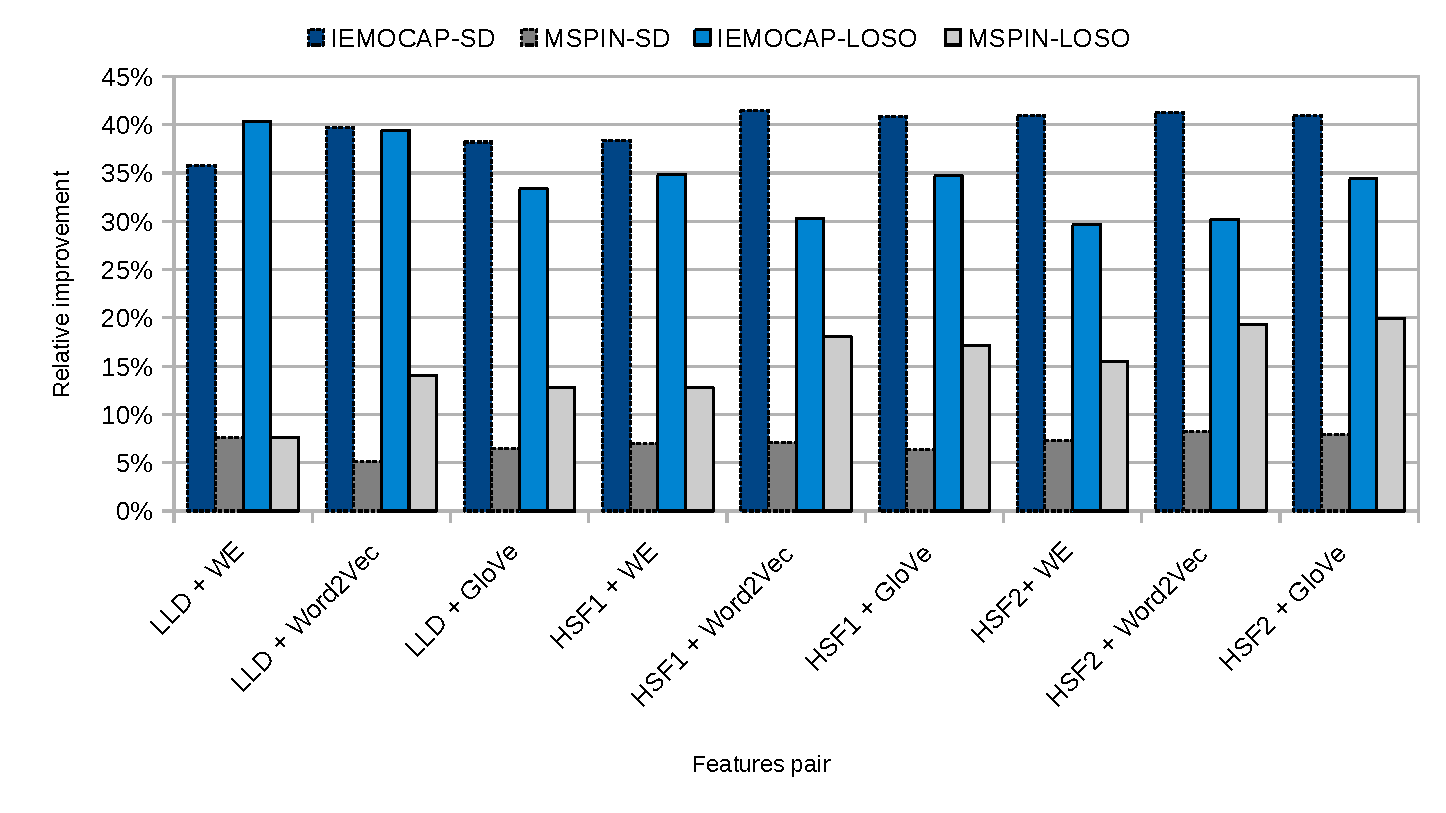
\includegraphics[width=\textwidth]{../fig/improvement.pdf}
\caption{Relative improvements in average CCC scores from the late fusion using
an SVM as compared to the highest average CCC scores from a single modality}
\label{fig:relative-improvement}
\end{figure}

\begin{table}[htpb]
\caption{Statistics of relative improvement by late fusion using an SVM as
compared to the highest scores for a single modality across datasets; the
scores were extracted from the data shown in Figure
\ref{fig:relative-improvement}.}   
\begin{center}
 \label{tab:relative-improvement}
 \begin{tabular}{l c c c c}
 \hline 
Statistic & IEMOCAP-SD & MSPIN-SD & IEMOCAP-LOSO & MSPIN-LOSO \\
\hline \hline
Average& 39.73\%   & 7.01\%    & 34.15\%   & 15.23\% \\
Max    & 41.45\%   & 8.22\%    & 40.32\%   & 19.93\% \\
Min    & 35.80\%   & 5.11\%    & 29.69\%   & 7.64\% \\
Std    & 1.90\%    & 0.93\%    & 3.84\%    & 3.90\% \\
 \hline
 \end{tabular}
\end{center}
\end{table} 

% todo: analysis speaker-dependent vs. speaker-independent
\subsection{Speaker-dependent vs. speaker-independent linguistic emotion recognition}
\label{subsect:sd_loso}
While speech-based emotion recognition is performed with a fixed random seed to
generate the same result for each run, linguistic-based emotion recognition
resulted in different scores for each run. The different results on linguistic
emotion recognition probably is caused by the initiation of weightings on
embedding layers. In this case, statistical tests can be performed on
linguistic emotion results to observe the difference between speaker-dependent
and speaker-independent scenarios. In contrast, statistical tests cannot be
performed between acoustic results and bimodal acoustic-linguistic results due
to the differences in the data (deterministic vs. non-deterministic). 

Table \ref{tab:test_sd_loso} shows if there is a significant difference between
speaker-dependent and speaker-independent results on the same feature set. The
$p-$value was set at 0.05 with a two-tail paired t-test between mean scores of
speaker-dependent and speaker-independent results. This paired t-test was based
on the assumption that there are no outliers (after pre-processing), and two
different inputs are fed into the same system. Only one result from linguistic
emotion recognition shows no significant difference in the IEMOCAP dataset. In
contrast, all results from the MSPIN dataset shows a significant difference
between speaker-dependent and speaker-independent results. This result reveals
a tendency for a difference in evaluating speaker-dependent and
speaker-independent data. The results from speaker-dependent data did not
represent speaker-independent data. In other words, results from
speaker-dependent data cannot be used to justify speaker-independent or whole
data.

\begin{table}
    \caption{Significant difference between speaker-dependent and speaker-independent scenarios on the same linguistic feature set; statistical tests were performed using two-tail paired $t-$test with $p-$value = 0.05.}
    \begin{center}
    \label{tab:test_sd_loso}
    \begin{tabular}{l c c}
        \hline
Feature     &   IEMOCAP     & MSPIN \\
\hline \hline
WE          &   Yes         & Yes   \\
word2vec    &   No          & Yes   \\
GloVe       &   Yes         & Yes   \\
    \hline
    \end{tabular}
    \end{center}
\end{table}

\subsection{Effect of removing target sentence from MSP-IMPROV dataset}
Since this research aims to evaluate the contribution of both acoustic and
linguistic information in affective expressions, it is necessary to have
sentences in the dataset that are free from any stimuli control. However, the
original MSP-IMPROV dataset contains 20 ``target'' sentences, the same sentence
that is elicited for different emotions (lexical-controlled data). These parts
of MSP-IMPROV dataset are irrelevant to this study; hence, it can be removed
from the dataset, i.e., \textit{Target - improvised} and \textit{Target - read}
parts. Nevertheless, it was found that the results show low CCC scores,
particularly on valence prediction, indicating the influences of the target
sentence. These results may be explained, as mentioned in section
\ref{subsect:svm_result}, that some of the utterances in the data analyzed in
this study also inadvertently included sentences semantically same as or
similar to those in the improvised target sentences (semi lexical-controlled
data). Hence, it is necessary to compare the contribution of linguistic
information in lexical-controlled and lexical-uncontrolled datasets, including
the threshold between these datasets.

\subsection{Final remarks}
A benchmark comparing this study with others is an ideal way to evaluate the
proposed method; however, no study has been found using the same dataset,
scenario, and metric for comparisons. Comparing to an early-fusion described in
the previous chapter, which reports an early fusion method on the IEMOCAP
dataset, this study improves the average CCC score from $0.508$ to $0.532$.
This higher result suggests that the late fusion is better than early fusion to
model bimodal acoustic-linguistic information fusion, which is in line with how
humans fuse multimodal information. This late-fusion approach can be embedded
with current speech technology, i.e., ASR, in which the text output can be
processed to weigh emotion prediction from acoustic features.

AbdelWahab and Busso \cite{Abdelwahab2018} used MSP-Podcast \cite{Lotfian2019},
collection of natural speech from audio-sharing website, as a target corpus
and IEMOCAP with MSP-IMPROV as source corpora to implement their DANN for
cross-corpus speech emotion recognition.  Although the goal is different, it
was observed similar patterns between theirs and the acoustic-only speech
emotion recognition int this study.  First, it was observed that the order of
the highest to the lowest CCC scores is arousal, dominance, and valence. This
pattern is also consistent when IEMOCAP is mixed with MSP-IMPROV as reported by
\cite{parthasarathy2017jointly} (in Table 2).  Second, it was observed that the
CCC scores obtained in IEMOCAP are higher than those obtained in MSP-IMPROV;
this lower score in MSP-IMPROV was due to the smaller size of the dataset. 

Along with the SVM architecture, this study also explored the parameters $C$
and $\gamma$, because both parameters are important for an RBF-kernel-based SVM
architecture \cite{scikit-learn}. Linear search was used in the ranges of
[$10^{-2}, 1, 10^2, 2 \times 10^2, 3 \times 10^2$] for $C$ and [$10^{-2},
10^{-1}, 1, 10, 10^2$] for $\gamma$ with a fixed value of $\epsilon$, i.e.,
0.01. The best parameter values were $C=200$ and $\gamma=0.1$. A repository has
been made to include the detailed implementation of the SVM architecture
\cite{Atmaja2020l}.

Per the stated objective in this chapter, this study applied two-stage
processing by using DNNs and an SVM for dimensional emotion recognition from
acoustic and linguistic features on four different datasets. It is found that
the combination of Mean+Std+Silence from the acoustic features and word
embeddings weighted by pre-trained GloVe embeddings achieved the highest result
among the nine pairs of acoustic-linguistic results from DNNs trained with
multitask learning. When the performance in obtaining one input to the SVM is
very low, the resulting relative improvement due to the SVM is also low. For
instance, the lowest improvement on MSPIN-LOSO was from LLD + WE features, in
which WE obtained a low score ($CCC_{avg}$ or $\overline{CCC}=0.136$) on
the linguistic network. This phenomenon suggests a challenging future research
direction for dealing with very little information, particularly linguistic
information, in the fusion strategy. One strategy applied in this research was
to use a pre-trained GloVe embedding on linguistic features with HSF2 on
acoustic features, which improved the $\overline{CCC}$ score from 0.358
(relative improvement = 7.64\%) to 0.422 (relative improvement = 19.93\%).
Other strategies should also be proposed, such as how to handle the data
differently when the same sentence elicits different emotions (i.e., whole
MSP-IMPROV dataset). In contrast, the current word-embedding feature treats the
same sentence as the same representation, even when it conveys different
emotions. Although BERT was used in the previous chapter, the configuration
only utilized a pre-trained model instead of fine-tuned model.


% comparing MSP-IMPROV vs. MSP-I+N i.e. comparing lexical-controlled vs.
% lexical-uncontrolled contents 
\section{Summary}
This chapter presents a late-fusion approach for acoustic-linguistic emotion
recognition. Several findings can be emphasized in this chapter. First, it was
found a linear correlation between the single-modality and late-fusion methods
in dimensional emotion recognition. The best result from each modality, when
they were paired, gave the best fusion result. Similarly, the worst result
obtained from each network, when they were paired, gave the worst fusion
result for bimodal emotion recognition. This finding differs from that
reported in \cite{Atmaja2019b}, which used an early-fusion approach for
categorical emotion recognition. In their work, the best pair differs from the
best methods in single modalities.

Second, linguistic features strongly influenced dimensional SER's score on the
valence dimension, while acoustic features strongly influenced arousal and
dominance scores. Accordingly, the proposed two-stage processing can take
advantage of linguistic features, which are commonly used in predicting
sentiment (valence) for the dimensional emotion recognition task. The proposed
fusion method improves all three emotion dimensions without attenuating the
performance of any dimension. The proposed method elevates scores of valence,
arousal, and dominance, subsequently from the highest to the lowest gain.

Third, the combination of input pairs does not matter in the proposed fusion
method, as indicated by the low deviation in relative improvement across the
nine possible input pairs. What does is the performance of the input in
the DNN stage. If the performance in the DNN stage is low
($\overline{CCC} \leq 0.2$), it will also result in low performance when paired
with another low-performance input in the SVM stage.

Future research can be directed to generalize the evaluated method presented in
this chapter for cross datasets --- different datasets are used for training and
test. While the SVM stage in this study only performed once, it can be extended
to be performed many times to observe such improvements. These broad research
directions are open challenges for researchers in speech emotion recognition.


% \newpage
% \thispagestyle{empty}
% \mbox{}
